%% The following macros taken from the CMS note
\newcommand{\MeV}{\ensuremath{\,\text{Me\hspace{-.08em}V}}\xspace}
\renewcommand{\gg}{\ensuremath{\PGg\PGg}\xspace}
\newcommand{\hgg}{\ensuremath{\PH\to\gg}\xspace}
\newcommand{\ggh}{\ensuremath{\Pg\Pg\PH}\xspace}
\newcommand{\vbf}{\ensuremath{\mathrm{VBF}}\xspace}
\newcommand{\vh}{\ensuremath{\mathrm{V}\PH}\xspace}
\newcommand{\tth}{\ensuremath{\Pqt\Pqt\PH}\xspace}
\newcommand{\zz}{\ensuremath{\PZ\PZ}\xspace}
\newcommand{\hzz}{\ensuremath{\PH\to\zz}\xspace}
\newcommand{\hzzllll}{\ensuremath{\hzz^{(\ast)}\to 4\ell}\xspace}
\newcommand{\ww}{\ensuremath{\PW\PW}\xspace}
\newcommand{\hww}{\ensuremath{\PH\to\ww}\xspace}
\newcommand{\hwwlnln}{\ensuremath{\hww^{(\ast)}\to\ell\Pgn\ell\Pgn}\xspace}
\newcommand{\bb}{\ensuremath{\PQb\PQb}\xspace}
\newcommand{\hbb}{\ensuremath{\PH\to\bb}\xspace}
\newcommand{\tautau}{\ensuremath{\Pgt\Pgt}\xspace}
\newcommand{\htt}{\ensuremath{\PH\to\tautau}\xspace}
\newcommand{\hlep}{\ensuremath{\PH\to\text{leptons}}\xspace}
\newcommand{\mumu}{\ensuremath{\PGm\PGm}\xspace}
\newcommand{\hmm}{\ensuremath{\PH\to\mumu}\xspace}
\newcommand{\wh}{\ensuremath{\PW\PH}\xspace}
\newcommand{\zh}{\ensuremath{\PZ\PH}\xspace}
\providecommand{\fbinv}{\mbox{\ensuremath{\,\text{fb}^\text{$-$1}}}\xspace}
\newcommand{\SM}{\ensuremath{\mathrm{SM}}\xspace}
\newcommand{\kZ}{\ensuremath{\kappa_{\mathrm{\PZ}}}\xspace}
\newcommand{\kW}{\ensuremath{\kappa_{\mathrm{\PW}}}\xspace}
\newcommand{\ktau}{\ensuremath{\kappa_{\PGt}}\xspace}
\newcommand{\ktop}{\ensuremath{\kappa_{\Pqt}}\xspace}
\newcommand{\kb}{\ensuremath{\kappa_{\Pqb}}\xspace}
\newcommand{\kmu}{\ensuremath{\kappa_{\Pgm}}\xspace}
\newcommand{\kglu}{\ensuremath{\kappa_{\mathrm{\Pg}}}\xspace}
\newcommand{\kgam}{\ensuremath{\kappa_{\PGg}}\xspace}
\newcommand{\GammaSM}{\ensuremath{\Gamma_{\PH}/\Gamma_{\PH}^{\mathrm{SM}}}\xspace}
\newcommand{\Bbsm}{\ensuremath{\mathrm{B_{BSM}}}\xspace}
\newcommand{\kV}{\ensuremath{\kappa_{\mathrm{V}}}\xspace}

In this section combination results are given for a parametrisation based on the coupling modifier, or $\kappa$-framework~\cite{Heinemeyer:2013tqa}. A set of coupling modifiers, $\vec\kappa$, is introduced to parametrize potential deviations from the SM~predictions of the Higgs boson couplings to SM~bosons and fermions. For a given production process or decay mode $j$, a coupling modifier $\kappa_j$ is defined such that,

\begin{equation}
\label{eq:kappa}
  \kappa_j^2=\sigma_j/\sigma_j^\SM\ \ \ {\rm or}\ \ \  \kappa_j^2=\Gamma^j/\Gamma^j_\SM.
\end{equation}

In the SM, all $\kappa_j$ values are positive and equal to unity. Six coupling modifiers corresponding to the tree-level Higgs boson couplings are defined: $\kW$, $\kZ$, $\ktop$, $\kb$, $\ktau$ and $\kmu$. In addition, the effective coupling modifiers $\kglu$ and $\kgam$ are introduced to describe \ggh production and \hgg decay loop processes. The total width of the Higgs boson, relative to the SM prediction, varies with the coupling modifiers as $\GammaSM = \sum_{j}\mathrm{B}^{j}_{\text{SM}}\kappa_{j}^{2} / (1 - \Bbsm)$, where $\mathrm{B}^{j}_{\text{SM}}$ is the SM branching fraction for the $\PH\rightarrow jj$ channel and $\Bbsm$ is the Higgs boson branching fraction to BSM final states. In the results for the $\kappa_j$ parameters presented here $\Bbsm$ is fixed to zero and only decays to SM particles are allowed. Projections are also given for the upper limit on $\Bbsm$ when this restriction is relaxed, in which an additional constraint that $|\kV| < 1$ is imposed. A constraint on $\GammaSM$ is also obtained in this model by treating it as a free parameter in place of one of the other $\kappa$ parameters.

The expected uncertainties for the coupling modifier parametrisation are summarised in Figure~\ref{fig:summary_K2} with numerical values given in Table~\ref{tab:summary_K2}. The largest uncertainty component is generally the signal theory in S1, whereas in S2 all four components contribute at a similar level for $\kgam$, $\kW$, $\kZ$ and $\ktau$. The signal theory remains the main component for $\ktop$ and $\kglu$, and $\kmu$ is limited by statistics.

Table~\ref{tab:summary_K2} also gives the expected uncertainties on $\Bbsm$ and $\GammaSM$ for the parametrisation with $\Bbsm\geq0$ and $|\kV|\leq1$. The $1\sigma$ uncertainty on $\Bbsm$ is $0.035$ in S1 and $0.027$ in S2, where in the latter case the statistical uncertainty is the largest component. The corresponding 95\% CL expected upper limit is $\Bbsm = 0.077 (0.057)$ in S1 (S2). The uncertainty on $\GammaSM$ is $0.05$ in S1 and $0.04$ in S2, equivalent to $0.16$ and $0.21\MeV$ respectively, assuming the SM width of $4.1\MeV$. The main contribution is the statistical uncertainty, followed by the experimental one.

\begin{figure}[hbtp]
\centering
% \includegraphics[width=0.5\textwidth]{\main/section2/plots/comb/summary_K2_300.pdf}%
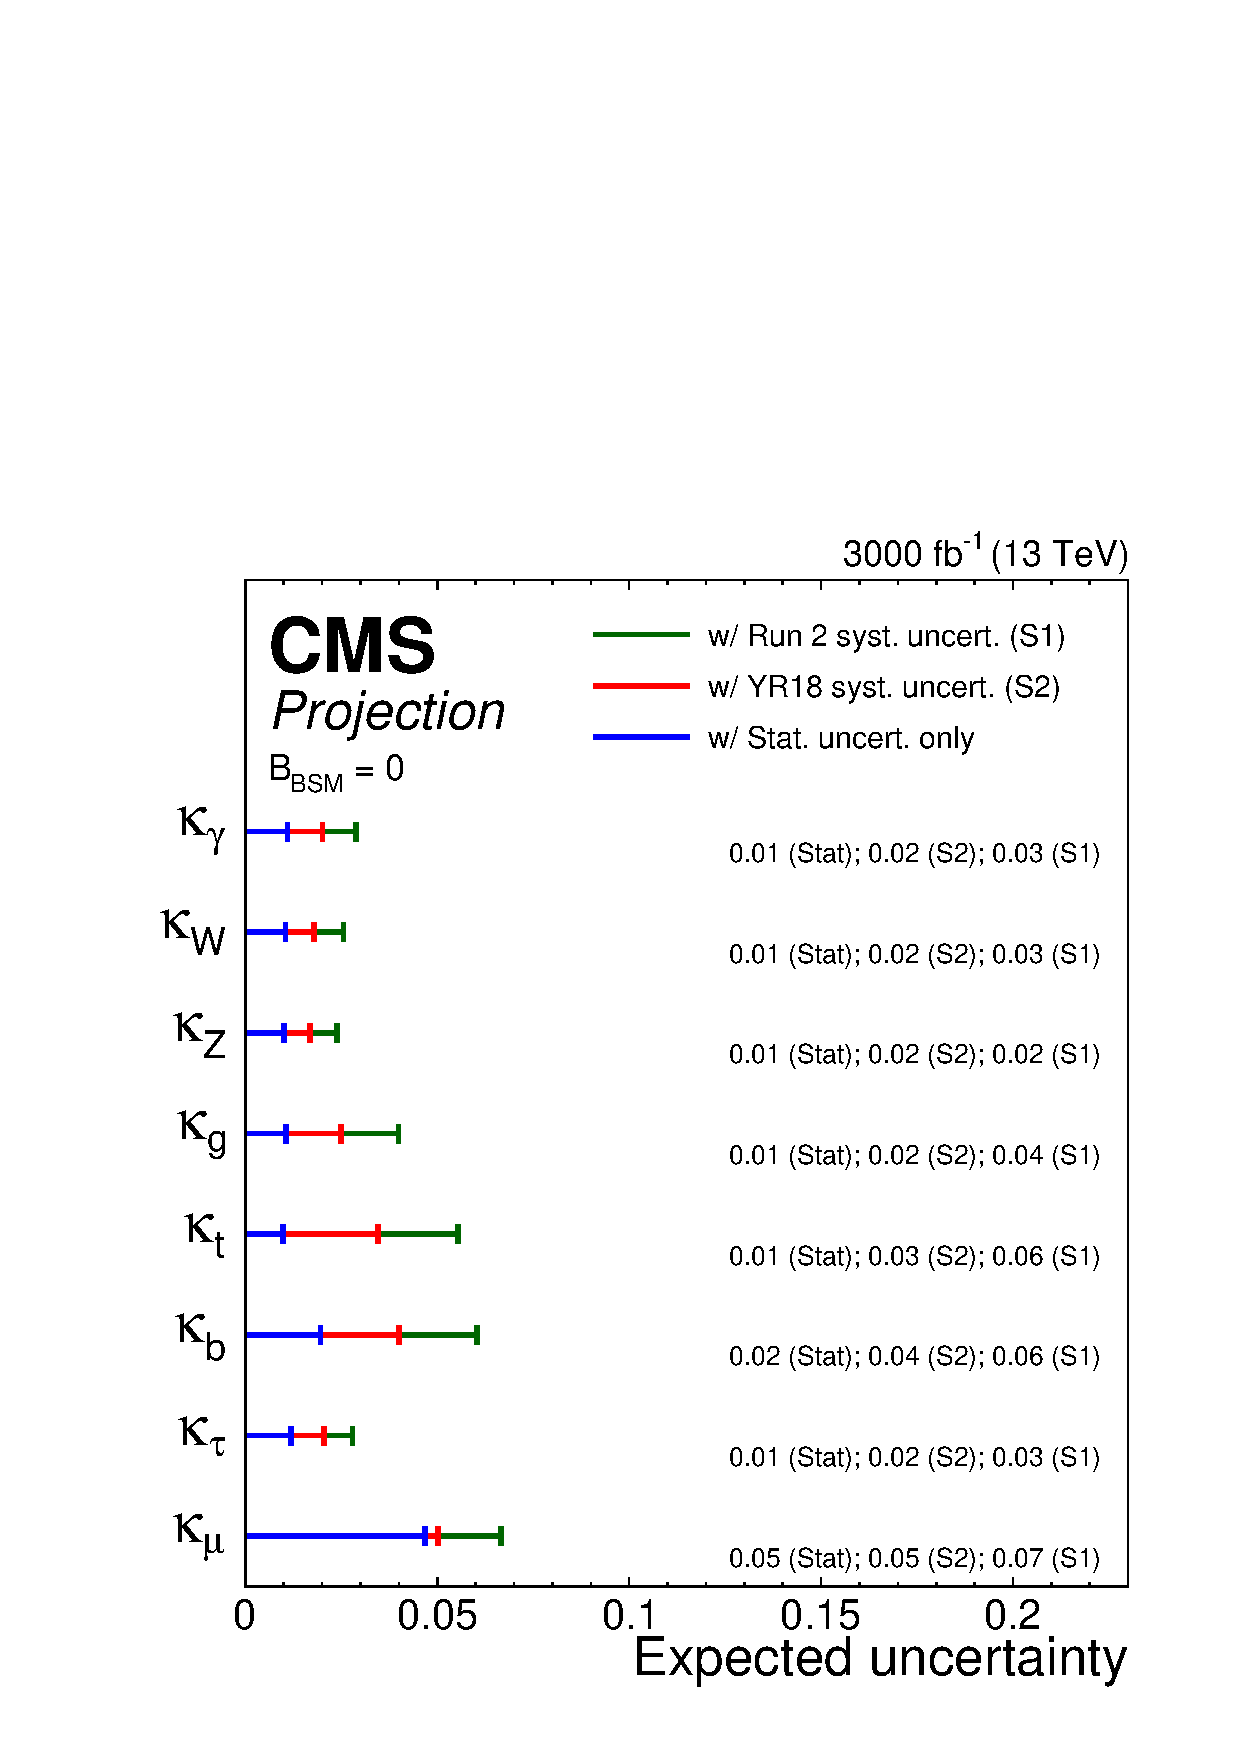
\includegraphics[width=0.6\textwidth]{\main/section2/plots/comb/summary_K2_3000.pdf}%
\caption{Summary plot showing the total expected $\pm 1\sigma$ uncertainties in S1 (with Run~2 systematic uncertainties~\cite{Sirunyan:2018koj}) and S2 (with YR18 systematic uncertainties) on the coupling modifier parameters. The statistical-only component of the uncertainty is also shown.}
\label{fig:summary_K2}
\end{figure}


\begin{table}[hbtp]
\centering
\caption{The expected $\pm 1\sigma$ uncertainties, expressed as percentages, on the coupling modifier parameters, as well as $\Bbsm$ and $\GammaSM$. Due to the constraint $\Bbsm \geq 0$ the values for this parameter correspond to the $+1\sigma$ uncertainties only.  Values are given for both S1 (with Run~2 systematic uncertainties~\cite{Sirunyan:2018koj}) and S2 (with YR18 systematic uncertainties). The total uncertainty is decomposed into four components: statistical (Stat), signal theory (SigTh), background theory (BkgTh) and experimental (Exp).}
\begin{tabular}{@{} l c c@{\hskip 0.15in} c c c c @{}}
 \hline
  &  & \multicolumn{5}{c}{3000 $\text{fb}^{-1}$} \\
  &  & Total & Stat & SigTh & BkgTh & Exp \\
  \hline
  \multicolumn{7}{c}{$\mathrm{B}_{\mathrm{BSM}} = 0$}\\
 \hline
\multirow{2}{*}{$\kappa_{\gamma }$} & S1  & 2.9& 1.1 & 1.8 & 1.0 & 1.7  \\[1pt]
                        & S2  & 2.0& 1.1 & 0.9 & 0.8 & 1.2  \\[4pt]
\multirow{2}{*}{$\kappa_{\mathrm{W}}$} & S1  & 2.6& 1.0 & 1.7 & 1.1 & 1.1  \\[1pt]
                        & S2  & 1.8& 1.0 & 0.9 & 0.8 & 0.8  \\[4pt]
\multirow{2}{*}{$\kappa_{\mathrm{Z}}$} & S1  & 2.4& 1.0 & 1.7 & 0.9 & 0.9  \\[1pt]
                        & S2  & 1.7& 1.0 & 0.9 & 0.7 & 0.7  \\[4pt]
\multirow{2}{*}{$\kappa_{\mathrm{g}}$} & S1  & 4.0& 1.1 & 3.4 & 1.3 & 1.2  \\[1pt]
                        & S2  & 2.5& 1.1 & 1.7 & 1.1 & 1.0  \\[4pt]
\multirow{2}{*}{$\kappa_{\mathrm{t}}$} & S1  & 5.5& 1.0 & 4.4 & 2.7 & 1.6  \\[1pt]
                        & S2  & 3.5& 1.0 & 2.2 & 2.1 & 1.2  \\[4pt]
\multirow{2}{*}{$\kappa_{\mathrm{b}}$} & S1  & 6.0& 2.0 & 4.3 & 2.9 & 2.3  \\[1pt]
                        & S2  & 4.0& 2.0 & 2.0 & 2.2 & 1.8  \\[4pt]
\multirow{2}{*}{$\kappa_{\tau }$} & S1  & 2.8& 1.2 & 1.8 & 1.1 & 1.4  \\[1pt]
                        & S2  & 2.0& 1.2 & 1.0 & 0.9 & 1.0  \\[4pt]
\multirow{2}{*}{$\kappa_{\mu}$} & S1  & 6.7& 4.7 & 2.5 & 1.0 & 3.9  \\[1pt]
                        & S2  & 5.0& 4.7 & 1.3 & 0.8 & 1.1  \\[4pt]
\hline
\multicolumn{7}{c}{$\mathrm{B}_{\mathrm{BSM}} \geq 0$, $|\kappa_{\mathrm{V}}| \leq 1$}\\
\hline
\multirow{2}{*}{$\mathrm{B}_{\mathrm{BSM}}$ \tiny{$(+1\sigma)$}} & S1  & 3.8& 1.9 & 2.4 & 1.5 & 1.7  \\[1pt]
                        & S2  & 2.7& 1.9 & 1.0 & 1.2 & 1.3  \\[4pt]
\multirow{2}{*}{$\Gamma/\Gamma_{\mathrm{SM}}$} & S1  & 5.8& 2.7 & 3.6 & 2.4 & 2.7  \\[1pt]
                        & S2  & 4.3& 2.7 & 1.9 & 1.8 & 2.1  \\[4pt]
\hline
\end{tabular}
\label{tab:summary_K2}
\vspace{0.5cm}
\end{table}

Figure~\ref{fig:corr_K2} gives the correlation coefficients for the coupling modifiers for S2. In contrast to the per-decay signal strength correlations in Figure~\ref{fig:corr_A1_5D} the correlations here are larger, up to $+0.74$. One reason for this is that the normalisation of any signal process depends on the total width of the Higgs boson, which in turn depends on the values of the other coupling modifiers. The largest correlations involve $\kb$, as this gives the largest contribution to the total width in the SM. Therefore improving the measurement of the $\hbb$ process will improve the sensitivity of many of the other coupling modifiers at the HL-LHC.

\begin{figure}[hbtp]
\centering
% \includegraphics[width=0.5\textwidth]{\main/section2/plots/comb/correlations_K2_S2_300.pdf}%
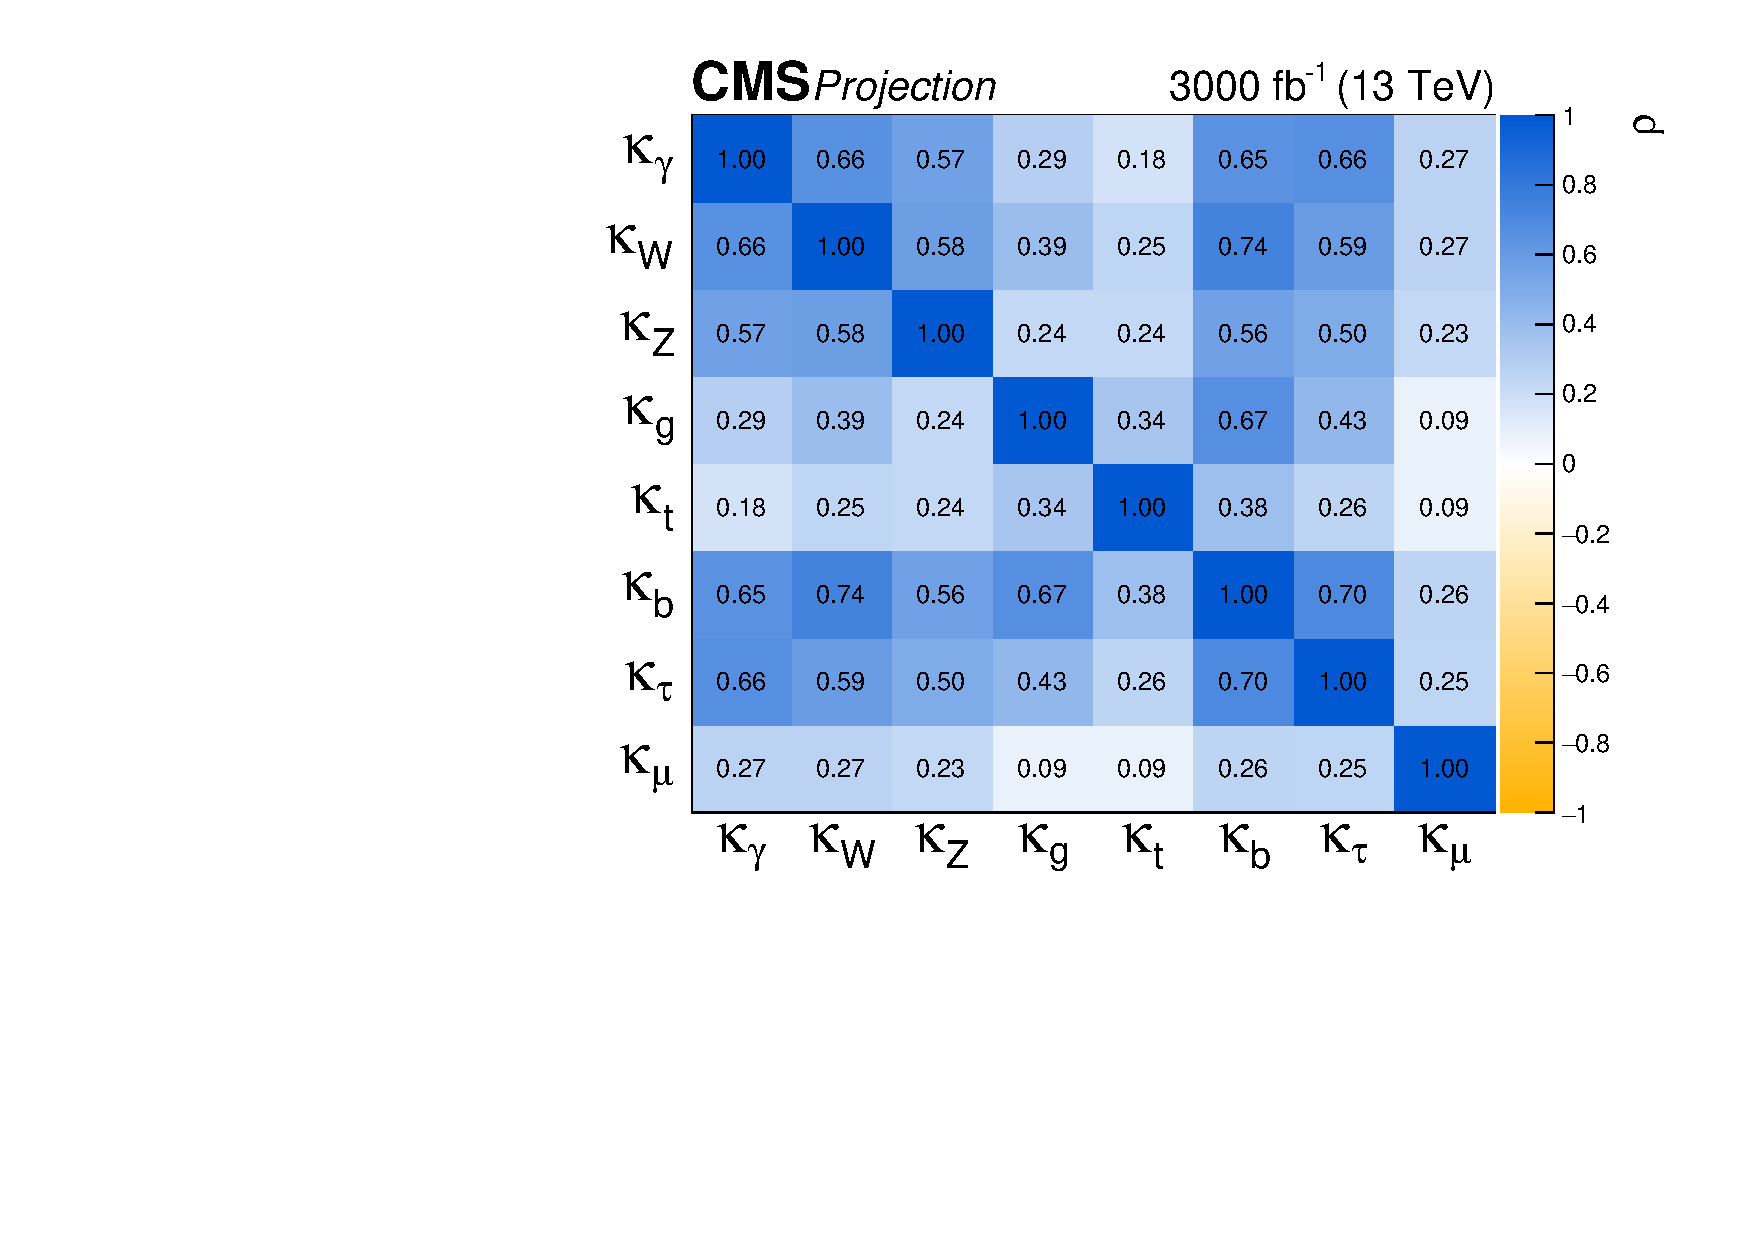
\includegraphics[width=0.6\textwidth]{\main/section2/plots/comb/correlations_K2_S2_3000.pdf}%
\caption{Correlation coefficients ($\rho$) between parameters in the coupling modifier parametrisation for S2 (with YR18 systematic uncertainties).}
\label{fig:corr_K2}
\end{figure}

% Projections have also been determined for an alternative parametrisation, based on ratios of the coupling modifiers ($\lambda_{ij} = \kappa_{i}/\kappa_{j}$). A reference combined coupling modifier is defined which scales the yield of a specific production and decay process. This is chosen to be $\kgluZ = \kglu\kZ/\kH$, where $\kH=\sum_{j}\mathrm{B}^{j}_{\text{SM}}$. The results of this projection are given in Appendix~\ref{sec:app-kappa-ratios}.